\section{Pengujian Performa Akselerator}
\label{sec:pengujian-performa-akselerator}

Pada pengujian performa akselerator \ac{RL}, terdapat dua komponen yang penting dilihat kecepatannya yaitu kecepatan pada tahap pembelajaran dan kecepatan pada tahap \textit{inference}. Pengujian kecepatan pada kedua tahap ini dilakukan menggunakan modul \textit{timer} yang dapat menghasilkan perbedaan \textit{clock cycles} dari hasil komputasi pada \textit{processor} VeeR EL2. Implementasi timer yang dibangun pada \textit{processor} VeeR EL2 merupakan adopsi dari spesifikasi OpenCores yang tersedia secara terbuka pada \parencite{open2024ptc}.

Modul timer tersebut, akan digunakan untuk menguji performa dua tahap sebagai berikut.

\begin{enumerate}
	\item Pembelajaran \acl{RL}\\
	      Pengujian ini akan mencoba membandingkan Algoritma \ref{alg:rl-qmemo} yang menggunakan perangkat lunak terhadap Algoritma \ref{alg:hw-sw-sep} yang menggunakan akselerator perangkat keras. Keduanya akan diuji pada \textit{processor} yang sama yaitu VeeR EL2.
	\item \textit{Inference} \acl{RL}\\
	      Pengujian ini akan mencoba membandingkan proses pemilihan aksi $a_{max}$ menggunakan metode eksploitasi. Perbandingan dilakukan dari perangkat lunak terhadap akselerator perangkat keras dengan instruksi q.max.
\end{enumerate}

Pada perbandingan performa \textit{inference}, hasil perbedaan waktu delay yang dibutuhkan oleh perangkat lunak dan akselerator akan diekstrapolasi untuk kasus \textit{cart pole balancing} dari sub-bab \ref{sec:rl-kontrol}. Tujuan akhirnya adalah agar dapat memperlihatkan dampak penggunaan akselerator pada suatu kasus fisis yang memerlukan kontrol secara \textit{real time}.

Pada pengujian tersebut, lingkungan pengujian permasalahan \textit{cart pole balancing} dilakukan menggunakan OpenAI Gymnasium \parencite{towers2023gymnasium}. Pada lingkungan OpenAI Gymnasium, permasalahan \textit{cart pole balancing} memiliki spesifikasi pada Tabel \ref{tab:state-space-cart-pole}.

\begin{table}[h!]
	\caption{Spesifikasi $State$ untuk \textit{Cart Pole Balancing} dari OpenAI Gymnasium}
	\label{tab:state-space-cart-pole}
	\centering
	\begin{tabular}{|c|c|c|}
		\hline
		Observation           & Min                             & Max                           \\
		\hline
		Cart Position         & -4.8                            & 4.8                           \\
		\hline
		Cart Velocity         & $-\infty$                       & $\infty$                      \\
		\hline
		Pole Angle            & $\sim -0.418$ rad $(-24^\circ)$ & $\sim 0.418$ rad $(24^\circ)$ \\
		\hline
		Pole Angular Velocity & $-\infty$                       & $\infty$                      \\
		\hline
	\end{tabular}
\end{table}

Dengan spesifikasi $state$ sesuai dengan Tabel \ref{tab:state-space-cart-pole}, permasalahan \textit{cart pole balancing} dari OpenAI Gymnasium memiliki aksi diskrit sebuah gaya $F$ dengan nilai yang fix, dengan pilihan pemberian gaya ke arah kiri atau kanan. Gambar \ref{fig:cartpole-openai} merupakan ilustrasi yang diberikan oleh OpenAI Gymnasium untuk lingkungan permasalahan \textit{cart pole balancing}.

\begin{figure}[h]
	\centering
	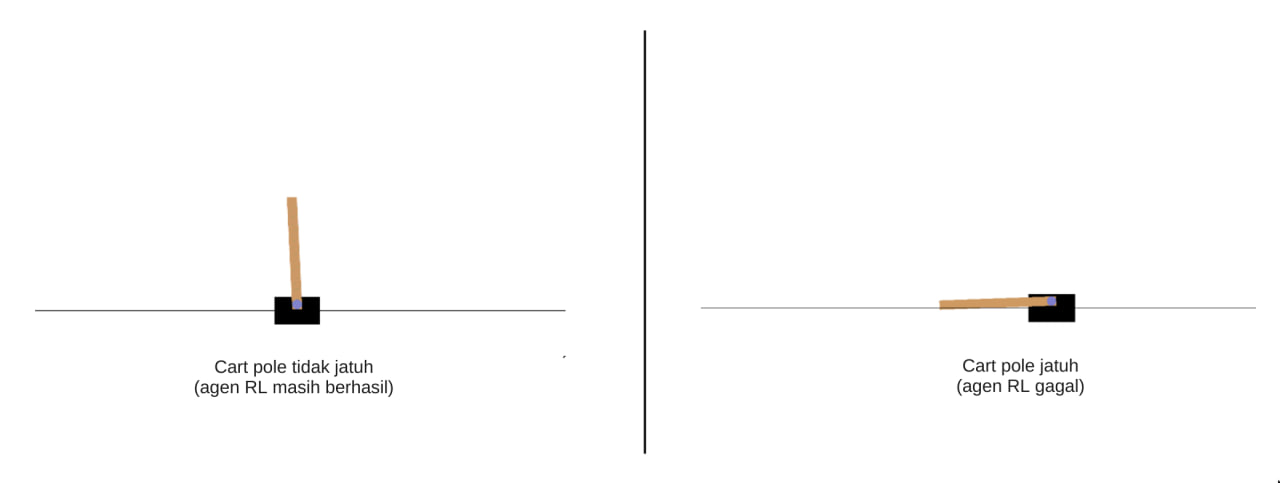
\includegraphics[width=1\textwidth]{chapter-3/cart-pole-openai.jpg}
	\caption{Ilustrasi Lingkungan Permasalahan \textit{Cart Pole Balancing} OpenAI}
	\label{fig:cartpole-openai}
\end{figure}

Tujuan dari lingkungan permasalahan pada Gambar \ref{fig:cartpole-openai} adalah agar terbentukan sebuah model agen \ac{RL} yang mampu menentukan arah gaya yang sesuai untuk setiap saat sehingga \textit{cart pole} tidak jatuh. Tentunya, delay dari komputasi akan sangatlah berpengaruh kepada pengambilan keputusan oleh agen \ac{RL}. Pada permasalahan di penelitian ini, aksi diskrit yang digunakan akan dibuat lebih besar, tidak hanya dua kemungkinan. Kemungkinan dari aksi diskrit akan diperpanjang dengan sebuah limit [$-F$, $F$] dengan pencacahan diskrit sehingga aksi menjadi sebanyak 1000 kemungkinan. Hal ini dilakukan untuk meninjau kemampuan akselerator untuk mengatasi permasalahan \textit{large branching factor} \parencite{amado2018qtable}.
